\chapter{Theoretical underpinning:\\Sensing-based interaction}\label{interaction}

\todo[inline]{Revision 5}

This chapter reviews theories in Human-Computer Interaction (HCI) to inform the design of computer interfaces to \emph{capture}, \emph{re-create} and \emph{generate} crisis training experience.

Field studies conducted by the author during physical simulations of crisis work (a description is available in Chapter \ref{research}) have identified requirements for the design of technologies to support each of the three stages derived from the CSRL model. Moreover focus groups with workers have highlighted the need for simple and intuitive user interfaces. To support the \emph{capture} stage the design goal emerged is to provide unobtrusive, distraction-free user interface to enable and control data collection. During \emph{re-creation} and \emph{generation} stages the objective is to provide situated, highly interactive user experiences using the captured data to promote reflection.

During field studies, the intrinsic physicality of crisis work was very visible. Contrarily to traditional office work, crisis work is often performed in harsh environments: workers deal with fire extinguishers, medical equipment, they break into crashed cars and houses falling apart. The physical environment is at the same time a source of danger, challenges and learning opportunities. Most of the activities are collaborative, e.g. carrying someone injured on a stretcher. Finally most of workers' were not used to ICT, and revealed little acquaintance with traditional user interfaces (point-and-click, touch-based, etc.).

When I started to design computer interfaces to support reflection for this very specific target group, it seemed to me advantageous to preserve some extent of \emph{physicality} into their user-experience with technology. While assisting the \emph{capture} of work experience the goal is to create technology which is unobtrusive because it blends into the (physical) work practice to become part of it; to support \emph{re-creation} and \emph{generation} of experiences technology should be engaging, enabling physical exploration of space and tangible interaction with digital information.

After surveying HCI literature for theoretical frameworks to facilitate integrating \emph{physicality} into computer interfaces I focused on the aspects of \emph{embodiment} and \emph{tangibility}. Those are characterising traits of sensing-based interfaces \autocite{Benford:2005bo}.

Sensing-based interfaces is rather a broad term referring to user interfaces that rely on sensor technology to make interaction between people and computers more intuitive and effective \autocite{Zhai:2005jm}. They allow for post-\textbf{WIMP} \autocite{VanDam:1997tz} interaction paradigms, to design user interfaces not relying on traditional \textbf{W}indows, \textbf{I}cons, \textbf{M}ouse and \textbf{P}ointers metaphors. Instead, sensing-based interfaces promote ``embodied interaction, tangible manipulation, physical representation of data and embeddedness in the real space'' \autocite{Hornecker:2006uq}. According to Rogers and Muller \autocite*{Rogers:2006te} sensing-based interaction allows the design of systems capable to deliver relevant information at appropriate times, which is critical to trigger and sustain reflection; and enable ``hands-free control'', which is fundamental for unobtrusively capturing data in action.

The theoretical tools to include \emph{embodiment} and \emph{tangibility} into user interfaces are reviewed in the next section.

\section{Tangible and mmbodied interaction}\label{tangible-interfaces-and-embodied-interaction}

Embodied interaction, as defined by Dourish \autocite{Dourish:2001vc}, is a collection of trends emerged in HCI, relying on the common ground to provide a natural user interaction with digital information. Embodied interaction makes an enormous shift from previous paradigms. Moving from time to space, it takes the interaction ``off the screen'' into the real world \autocite{Dourish:2001vc}; distributing inputs in space, de-sequentialising interaction and reducing the gap between where the information is created where it is accessed. The interactional media, with its affordances, is the interface: ``By treating the body of the device as part of the user interface --an embodied user interface-- we can go beyond the manipulation of a GUI (Graphical User Interface) and allow the user to really directly manipulate an integrated physical-virtual device'' \autocite{Fishkin:2000df}

Tangible user interfaces (TUIs) are computer interfaces in which technology is embedded into physical objects and spaces, enabling an embodied interaction with digital information. In this picture, unlike GUIs which manipulate virtual elements (e.g.~icons) with the aid of keyboard and mouse, TUIs integrate both representation and control of computation into physical artefacts \autocite{krumm2009ubiquitous}. This approach allows system designers to be free to experiment with new type of metaphors, taking advantage of users' physical skills and providing interfaces which exploit people's knowledge with the everyday, non-digital, world \autocite{Jacob:2008vm}. Since the ways the manipulation of physical media profoundly differs from the manipulation of the digital \autocite{Terrenghi:2007uv}, metaphors adopted for the digital world need to be redesigned to meet physical affordances. The design of TUIs as well as other sensing-based interfaces poses new challenges to designers \autocite{Bellotti:2002wg}. Those challenges were also further elaborated by Marquardt and Greenberg \autocite*{Marquardt:2012tg}. Several terms have been used to characterise systems of tangible interfaces: e.g. \emph{tangibles}, \emph{graspables}, \emph{tokens}, \emph{containers}, \emph{phicons}, \emph{tangible bits}; in the following I will call them \emph{tangibles}.

\emph{Tangibles} are part of the broad field known as Ubiquitous Computing, widely attributed to the work of Mark Weiser. In his pioneering article on Scientific American \autocite{weiser1991computer} he envisioned a close coupling between the digital and the physical, to the extent that the technology ``disappears into the fabric of the everyday life''.

\subsection{Theoretical frameworks}\label{frameworks}

Over the years several research initiatives have proposed frameworks either to characterise systems of tangibles, e.g. \autocites{Fishkin:2004uv}{Jacob:2008vm}{Hornecker:2006uq}; or to provide opportunities and guidelines to support the design of new TUIs, e.g. \autocites{Benford:2005bo}{Shaer:2004ta}{Rogers:2006te}.

In 2000, Ullmer and Ishii \autocite*{Ullmer:2000vf} took the first steps investigating the design of tangibles. They defined TUIs as computer interfaces that give physical form to digital information, rethinking the interfaces itself as being composed by some sort of ``tangible bits'' \autocite{Ishii:2008fh}. In order to help understanding and building tangibles, they created a conceptual framework and interaction model called MCRit. MCRit, an abbreviation for Model-Control-Representation (tangible and intangible), adapts the Model-View-Controller (MVC) model of GUI-based interaction to the design of tangibles. Besides MCRit highlights the ``seamless integration of control and representation'' characteristic of tangibles, it redefines the capability of the interface to provide information as a balance between its physical representation (the object's shape and affordances) and a intangible one (e.g.~computer graphics and sounds) (Figure \ref{fig:mcrit-model}). For example by augmenting physical objects with video-projections and sounds in order to extend the static representation of an object with an intangible, dynamic one.

\begin{figure}
	[tbh] \centering 
	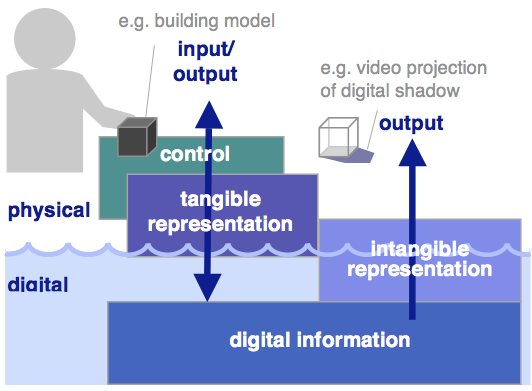
\includegraphics[width=0.75
	\textwidth]{mcrit} \caption{Tangible and intangible representations of TUI. Figure adapted from \protect\autocite{Ishii:2008fh}} \label{fig:mcrit-model} 
\end{figure}

In fact one of the main pitfalls of TUIs is that while GUIs serve as generic purpose interfaces by allowing multiple kinds of tasks, defined by the software; TUIs serve as special purpose interfaces, each one tailored to a specific set of actions (defined by physical affordances and constrains). A tangible interface can hardly be adapted to work in a context that differs from the one it has been designed for. This trade-off has been defined by Jacob \autocite*{Jacob:2008vm} between Reality and Versatility: it trades the capability of a system of doing many different tasks (like browsing photos, writing a document) with the possibility to accomplish only one single task with a higher level of realism or simplicity.

Following the work of Ullmer and Ishii other research has looked at tangibles from other perspectives. Jacob et al. \autocite*{Jacob:2008vm} identifies four interaction themes with the real world that can be leveraged for the design of TUIs. Hornecker and Buur \autocite*{Hornecker:2006uq} present four topics to be considered in scenarios where tangible interaction has social aspects. Fishkin \autocite{Fishkin:2004uv} presents an aggregated perspective on other frameworks, categorising tangible systems as a continuum spectrum according to the level of embodiment and metaphor they provide. Finally Ullmer et al. \autocite{Ullmer:2005jz} envision TUIs as a systems of \emph{tokens} and \emph{constraints}. The former are discrete physical objects that represent digital information, the latter mechanical or visual confining regions that are mapped to digital operations. By the interaction phases of association and manipulation of tokens within a system of constraints it is possible to map physical actions to a set of computational operations in a grammar of ways. For example the presence or absence of a token in a constrained area could be easily digitalised in binary information to trigger a digital operation. For a literature review on other frameworks see \autocite{Mazalek:2009uy} and \autocite{Shaer:2009fx}.

\subsection{Applications in reflective learning}\label{applications-of-tangibles-in-reflective-learning}

Although the relation between tangibles and reflective learning has not been thoroughly investigated, several works have shown that TUIs might be beneficial for learning \autocite{Marshall:2007dr}; for a review see \autocite{omalley:hal-00190328}. Although these often focus on applications of TUIs for children and classroom environments, TUIs might have possible benefits on learning on a broader scope. Those benefits include the support to more natural \autocite{Terrenghi:2005gq} and situated \autocite{Klemmer:2006ez} learning, and increased reflection and engagement \autocite{Rogers:2006te} due to the link between physical action and digital feedbacks. Moreover TUIs foster collaboration \autocite{Rogers:2003tt}, in which they increase visibility of others' actions and allow for concurrent interaction.

Theoretical tools adapted from the presented frameworks have driven the design of sensing-based interfaces described in Chapter \ref{results}.

In the next chapter I will present the research methodology adopted throughout the work, providing details on the field studies performed and prototypes built. 
